\documentclass{article} % For LaTeX2e
\usepackage{nips15submit_e,times}
\usepackage{hyperref}
\usepackage{url}
\usepackage{graphicx}
\usepackage{subcaption}
\usepackage{amsthm}
\usepackage{algorithm}
\usepackage[noend]{algpseudocode}

\theoremstyle{definition}
\newtheorem{definition}{Definition}[section]
\newtheorem{theorem}{Theorem}[section]
\newtheorem{corollary}{Corollary}[theorem]
\newtheorem{lemma}[theorem]{Lemma}
\newtheorem{assumption}{Assumption}
%\documentstyle[nips14submit_09,times,art10]{article} % For LaTeX 2.09
\title{}
\author{}
\newcommand{\fix}{\marginpar{FIX}}
\newcommand{\new}{\marginpar{NEW}}
\nipsfinalcopy % Uncomment for camera-ready version
\begin{document}

\maketitle

\begin{abstract}

\end{abstract}

\section{Definitions}

\begin{definition}[Markov Property]
A stochastic process has the Markov property if the conditional
probability distribution of future states of the process (conditional
on both past and present states) depends only upon the present state,
not on the sequence of events that preceded it.
\[
P(x_{n+1} | x_{n}, x_{n-1}, \dots, x_{1}) = P(x_{n+1} | x_{n})
\]
\end{definition}

\begin{definition}[k-order Markov Chain]
A Markov chain of order $k$ has the property that:
\[
P(x_{n+1} | x_{n}, x_{n-1}, \dots, x_{1}) = P(x_{n+1} | x_{n}, \dots, x_{n-(k-1)})
\]
The future state $x_{n+1}$ depends on the past $k$ states. Remembering
$k$ states restores the Markov property and a larger memory grants no
further predictive power.
\end{definition}

\begin{definition}[Entropy]
The entropy of a discrete random variable $X$ with alphabet $\mathcal{X}$ is
defined by:
\[
H(X) = \sum_{x\in \mathcal{X}} p(x) \log p(x)
\]
\end{definition}

\begin{definition}[Mutual Information]
The mutual information between two random variables $I(X;Y)$ is the
reduction of uncertainty of $X$ due to knowledge of $Y$:
\[
I(X;Y) = \sum_{x,y} p(x,y) \log \frac{p(x|y)}{p(x)} = H(X) - H(X|Y)
\]
\end{definition}

\section{Partial Observability}
In the context of reinforcement learning, partial observability
describes the category of agent-environment interactions in which an
agent's perceptions do not provide complete information about the true
state of the environment. This problem is also known as
\textit{incomplete perception}, \textit{perceptual aliasing}, or
simply \textit{hidden state}.

One cause of partial observability is sensor noise, in which two
different states appear to be the same state due to noise in
observations. Another cause is perceptual aliasing, in which multiple
environment states are indistinguishable given the
observations. Figure \ref{fig:functions} illustrates these cases.

\begin{figure}[htp]
\centering
\begin{subfigure}{.3\textwidth}
  \centering
  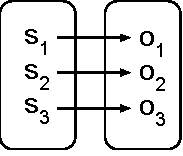
\includegraphics[width=.6\linewidth]{figures/bijection}
  \caption{Fully Observed}
  \label{fig:bijection}
\end{subfigure}
\begin{subfigure}{.3\textwidth}
  \centering
  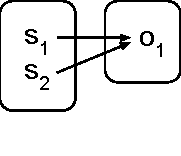
\includegraphics[width=.6\linewidth]{figures/state-aliasing}
  \caption{State Aliasing}
  \label{fig:state-aliasing}
\end{subfigure}
\begin{subfigure}{.3\textwidth}
  \centering
  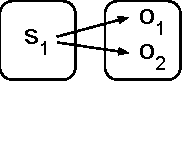
\includegraphics[width=.6\linewidth]{figures/noisy-perception}
  \caption{Noisy Perceptions}
  \label{fig:noisy-perception}
\end{subfigure}
\caption{A fully observed environment features an injective mapping
  from true states to observations. Partial observability indicates
  the degree to which this injection is invalid. Two sources of
  partial observability are state aliasing, the degree to which the
  observation function is non-injective, and noisy perceptions, the
  degree to which the observation function is not a valid function.}
\label{fig:functions}
\end{figure}

\subsection{Criteria for Partial Observability}
\begin{assumption}
The underlying behavior of the environment operates according to a
Markov Decision Process. In particular, the environment features a
true state for which the Markov property holds.
\end{assumption}

The following conditions are necessary and sufficient for an
environment to be considered partially observable:

\begin{enumerate}
\item The environment provides observations rather than true states.
\item The mapping from true states to observations not injective (one-to-one).
\end{enumerate}

The non-injectivity in the mapping between true states and
observations determines the degree of partial observability.

\section{An Information-Theoretic View of Partial Observability}
One way to understand the partial observability of a domain is to
quantify the amount of information the observations provide about the
true states. Let us assume we have access to the true environment
state which generates each observation. Let $S$ be a random variable
over the domain of all possible states, and $O$ be a random variable
over all possible observations. The mutual information $I(S;O)$
computes the reduction in uncertainty of the true environment states
$S$ resulting from knowledge of the observations $O$:

\[
I(S;O) = \sum_{s,o \in S \times O} p(s,o) \log \frac{p(s|o)}{p(s)} = H(S) - H(S|O)
\]

If the mapping from states to observations is one-to-one, the mutual
information $I(S;O)$ will equal $H(S)$, and the agent's interaction
with the environment is said to be fully observed.

\section{Using a History of Observations}
A natural technique to deal with partial observability is to augment
the agent's state representation to include a history of
observations. This strategy helps to address state aliasing by using
the observation history to disambiguate aliased states. In the case of
noisy observations, a history could be used to counteract noise, for
example by computing an average. However, the size of the state space
grows exponentially as a function of history length, so in practice it
is rarely feasible to maintain extensive history.

\begin{definition}[k-th Order Mutual Information]
Let $\textbf{O}^k$ be a random variable over the domain of all
k-length observation sequences $\textbf{o}^k = (o_t, o_{t-1}, \dots,
o_{t-(k-1)})$. We define the $k$-th order mutual information between
$k$-length observation histories and true states as follows:

\[
I(S;\textbf{O}^k) = \sum_{s,\textbf{o}^k \in S \times \textbf{O}^k} p(s_t,\textbf{o}^k) \log \frac{p(s|\textbf{o}^k)}{p(s)}
\]
\end{definition}

The growth of $I(S;\textbf{O}^k)$ as a function of $k$ reveals the
predictive power gained by leveraging additional history. Even
maintaining a full history cannot guarantee full observability in all
cases: in an extreme case where all states are mapped to the state
observation, even a full history is no help in predicting the next
state.

%% \begin{algorithm}
%% \caption{My algorithm}
%% \label{euclid}
%% \begin{algorithmic}
%% \If {$i\geq maxval$}
%%     \State $i\gets 0$
%% \Else
%%     \If {$i+k\leq maxval$}
%%         \State $i\gets i+k$
%%     \EndIf
%% \EndIf
%% \end{algorithmic}
%% \end{algorithm}

\section{Atari Games}



\begin{definition}[Observability]
Assuming access to the true state distribution $S$ of an environment
as well as the observation distribution $O$, the observability
$\mathcal{O}$ of the environment is given by conditional entropy of
the true states given the observations, divided by the entropy of the
states.
\[
\mathcal{O} = 1 - \frac{H(S|O)}{H(S)}
\]
The observability quantifies how much information the observations
possess about the true environment state. Observability is always
between zero and one: an observability of zero indicates the
observations are no help in understanding the environment's state. An
observability of one implies the observations fully determine the true
state. Observability measure the degree of bijectivity in an
environment's mapping from states to observations.
\end{definition}


\section{Half Baked Ideas}
The following sections contain intuitions that may have some promise
but are poorly grounded.

\section{Sub-optimality induced by partial observability}
Partial observability causes agents to learn sub-optimal policies. The
degree of partial observability inherent in an environment bounds the
performance of an optimal policy learned over observations $\pi_O^*$
compared to the optimal policy learned over true states $\pi_S^*$:
\[
\textrm{sub-optimality} \propto \sum_{s\in S} D_{KL}\big(\pi_O^*(O(s))\ ||\ \pi_S^*(s)\big)
\]

\end{document}
